%\documentclass[11pt,letterpaper]{article}
\documentclass[14pt,letterpaper]{extarticle}

% ----------------------------------
%            PAQUETES
% ----------------------------------
\usepackage[spanish]{babel}
\usepackage[utf8]{inputenc}
\usepackage[T1]{fontenc}
\usepackage{lmodern}  
\usepackage{csquotes}
\usepackage{setspace}           % Interlineado
\usepackage{geometry}           % Márgenes

							          % Hipervínculos
\usepackage{titlesec}           % Formato de títulos
\usepackage{tocloft}            % Formato de tabla de contenido
\usepackage{filecontents}
\usepackage{graphicx}
\usepackage{apacite}            % Estilo APA
\usepackage{indentfirst}        % Sangría en primer párrafo


\onehalfspacing                 % Interlineado 1.5
\graphicspath{{./Imagenes/}}
\usepackage{float}
\restylefloat{figure}
\usepackage{amsmath}



% ----------------------------------
%            FORMATO APA
% ----------------------------------
\geometry{left=2.54cm, right=2.54cm, top=2.54cm, bottom=2.54cm}
\onehalfspacing     % Interlineado 1.5

% Estilo de títulos APA
\titleformat{\section}{\normalfont\bfseries\large}{\thesection.}{0.5em}{}
\titleformat{\subsection}{\normalfont\bfseries\normalsize}{\thesubsection.}{0.5em}{}

% ----------------------------------
%        PORTADA TIPO APA
% ----------------------------------
\title{\textbf{Título del Informe}}
\author{Marlon Iván Carreto Rivera}
\date{\today}


\usepackage{pdfpages}
\usepackage{hyperref} 
\hypersetup{
	colorlinks=true,
	linkcolor=black,
	urlcolor=black,
	citecolor=black
}









% ----------------------------------
\begin{document}
	
		
\includepdf[pages=-,pagecommand={}]{Caratula/Caratulaanteproyecto.pdf}
	%%
\includepdf{Caratula/Caratulaanteproyecto.pdf}
	%\maketitle
	\thispagestyle{empty}


	\newpage
	
	
	
	
	
	
	% ----------------------------------
	%      TABLA DE CONTENIDO
	% ----------------------------------
	\renewcommand{\contentsname}{Contenido}
	\tableofcontents
	\newpage
	

	
	% ----------------------------------
	%        CONTENIDO DEL INFORME
	% ----------------------------------
	
	\section*{Introducción }
	
	% --- Introducción (sin numerar, con link funcional) ---
	\phantomsection
	\addcontentsline{toc}{section}{Introducción}
	El presente documento da a conocer  la clasificación de las obras ya que adquiere gran importancia, que permite establecer el nivel de relevancia  y el desempeño esperado de cada edificación o  construcción. De igual forma, la correcta identificación y evaluación de las cargas que actúan sobre una edificación, tanto gravitacionales como sísmicas, constituyen la base para un diseño estructural adecuado.
	
	Además, la normativa enfatiza la necesidad de analizar las irregularidades en planta y en elevación, debido a que estas pueden alterar el comportamiento dinámico de la estructura durante un sismo, incrementando su vulnerabilidad si no se consideran apropiadamente.
	
	Por otro lado, la redundancia estructural representa un principio esencial dentro del diseño sismo-resistente, ya que mejora la capacidad de la estructura para redistribuir esfuerzos y evita la ocurrencia de fallas progresivas.
	

	
	
	
		\newpage
	% ----------------------------------

	
	\section{Clasificación de Obras}
	
	La normativa guatemalteca, a través de las \textbf{Normas de Seguridad Estructural para Guatemala (AGIES)}, establece una categorización estricta para todas las edificaciones e infraestructura del país. Esta clasificación se fundamenta principalmente en el \textbf{uso previsto de la estructura}, el \textbf{nivel de ocupación (número de personas)} y la \textbf{importancia estratégica} de la obra para la atención y recuperación de la comunidad inmediatamente después de la ocurrencia de un evento sísmico mayor u otro desastre natural.
	
	De acuerdo con el documento normativo analizado, las obras se subdividen en cuatro grandes categorías obligatorias (Categorías I a IV), las cuales definen las demandas sísmicas de diseño mediante el factor de combinación de carga y los requerimientos de supervisión técnica 
	
	\subsection{Categoría I: Obras Utilitarias o Menores}
	Esta categoría comprende aquellas estructuras que presentan un riesgo muy bajo para la vida humana en caso de fallo, debido a su baja ocupación o carácter temporal  Generalmente, son obras accesorias que no están destinadas a la habitabilidad continua de personas.
	
	\begin{itemize}
		\item \textbf{Descripción:} Edificaciones aisladas o complementarias cuya falla estructural no compromete la seguridad de servicios públicos ni de estructuras adyacentes de mayor importancia 
		\item \textbf{Ejemplos típicos:} Bodegas agrícolas de almacenamiento temporal, muros de cerramiento perimetral, cobertizos de herramientas, invernaderos menores, instalaciones provisionales de obra y viviendas unifamiliares mínimas de un solo nivel construidas con materiales ligeros.
	\end{itemize}
	
	\begin{figure}
		\centering
		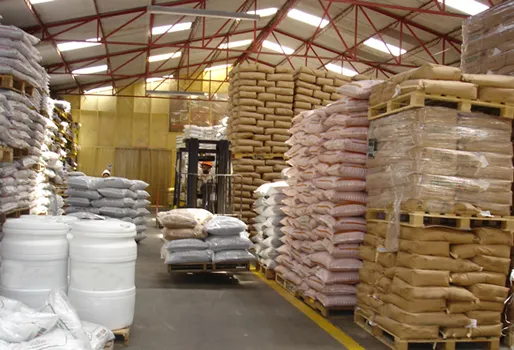
\includegraphics[width=0.7\linewidth]{im1}
		
		\label{fig:im1}
	\end{figure}
	
	
	
	
	
	\subsection{Categoría II: Obras Ordinarias o Convencionales}
	Representa el estándar común de las edificaciones urbanas y habitacionales. Incluye a todas las estructuras destinadas a vivienda, comercio o trabajo que albergan densidades normales de población y cuya falla, aunque trágica, tiene un impacto social localizado 
	
	\begin{itemize}
		\item \textbf{Descripción:} Edificios de uso residencial, comercial o industrial que no clasifican en las categorías de alta ocupación (III) ni en las esenciales de emergencia (IV) 
		\item \textbf{Ejemplos típicos:} Casas de habitación familiares de uno o más niveles, edificios de apartamentos residenciales convencionales, hoteles estándar, oficinas corporativas, locales comerciales individuales, restaurantes, gasolineras, cárceles o centros de detención, e instalaciones industriales destinadas a manufactura ligera.
	\end{itemize}
	
	
	\begin{center}
		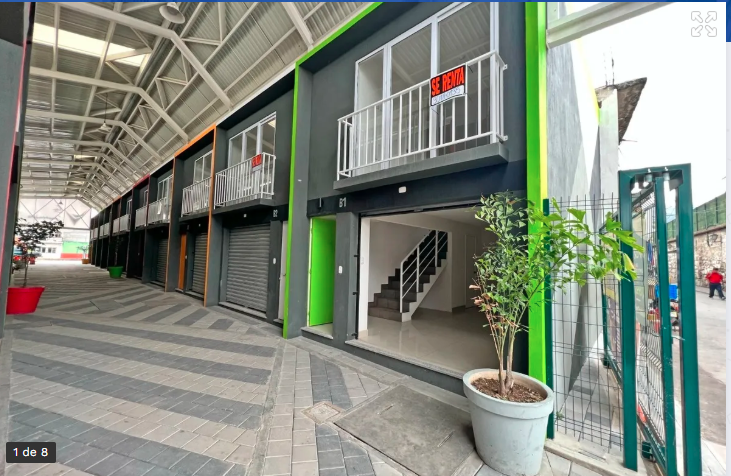
\includegraphics[width=0.7\linewidth]{im2}
	\end{center}
	
	
	
	
	\subsection{Categoría III: Obras Importantes o de Alta Ocupación}
	En este grupo se clasifican las estructuras que albergan de forma continua o temporal a una \textbf{gran cantidad de personas}, o bien, aquellas que resguardan bienes de un valor cultural, histórico o económico extraordinario para la nación . El diseño sísmico de estas obras es más exigente debido al alto costo social que implicaría su colapso ..
	
	\begin{itemize}
		\item \textbf{Descripción:} Edificaciones públicas o privadas con capacidades masivas de reunión, o que contienen sustancias de peligrosidad moderada.
		\item \textbf{Ejemplos típicos:} 
		\begin{itemize}
			\item Centros educativos (escuelas, colegios, universidades y guarderías).
			\item Centros de reunión masiva con capacidades que exceden los límites ordinarios (cines, teatros, estadios, auditorios, iglesias y templos de gran afluencia).
			\item Centros comerciales de gran escala (Malls) y terminales de transporte de pasajeros.
			\item Museos, archivos nacionales y edificios gubernamentales de atención masiva al público.
			\item Instalaciones de almacenamiento de sustancias e insumos industriales tóxicos o explosivos que no sean considerados críticos de seguridad nacional.
		\end{itemize}
	\end{itemize}
	
	
	\begin{center}
		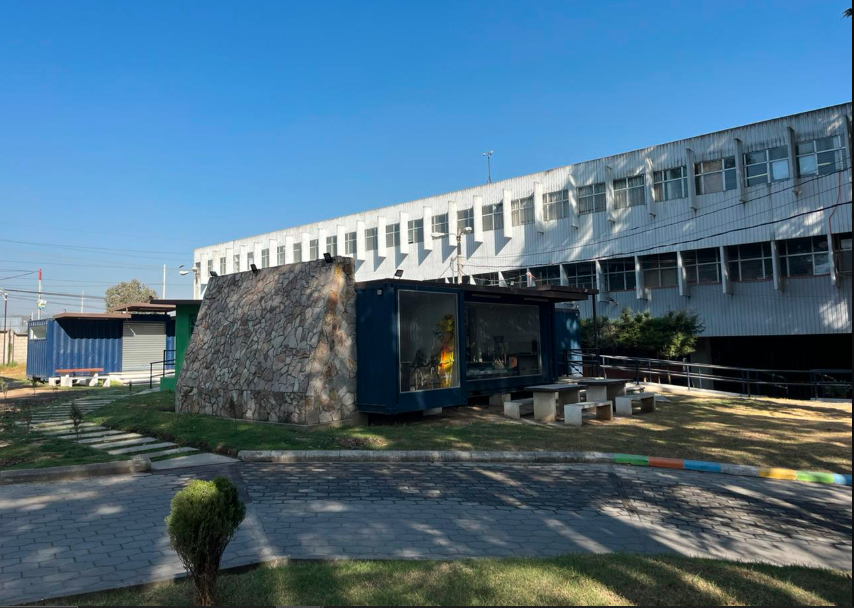
\includegraphics[width=0.7\linewidth]{im3}
	\end{center}
	
	
	
	
	
	\subsection{Categoría IV: Obras Esenciales}
	Esta categoría es la más crítica dentro de la planificación de resiliencia ante desastres en Guatemala. Comprende aquellas edificaciones que \textbf{deben permanecer operativas e intactas durante y después de un sismo severo} para coordinar las operaciones de rescate, atención médica de emergencia y mantenimiento del orden público ..
	
	\begin{itemize}
		\item \textbf{Descripción:} Infraestructura y centros de comando indispensables para la mitigación del desastre, la atención post-evento de la población civil y la continuidad del Estado ..
		\item \textbf{Ejemplos típicos:}
		\begin{itemize}
			\item Hospitales de alta complejidad, centros de salud con servicios de cirugía de emergencia y clínicas de trauma ..
			\item Estaciones de bomberos, sedes centrales de la policía nacional civil y recintos militares estratégicos ..
			\item Centros de operaciones de emergencia (como las instalaciones de la CONRED), centros de telecomunicaciones nacionales, antenas de transmisión de señales de emergencia y torres de control de tráfico aéreo ..
			\item Infraestructura de servicios públicos vitales: plantas de tratamiento y bombeo de agua potable, subestaciones eléctricas principales y centrales de generación de energía ..
			\item Refugios designados para emergencias y hangares de aeronaves de rescate.
		\end{itemize}
	\end{itemize}
	
\begin{center}
	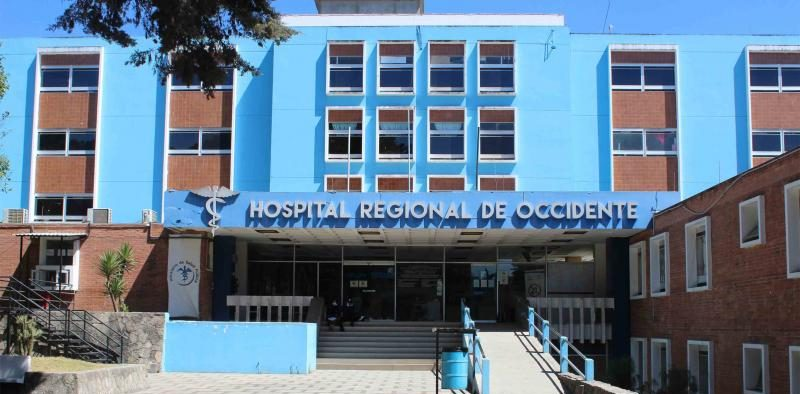
\includegraphics[width=0.7\linewidth]{im4}
\end{center}

	
	
	
	
	
	\subsection{Implicaciones de la Clasificación en el Diseño Estructural}
	La asignación de una obra a una de estas categorías altera directamente los parámetros del modelo de cálculo ingenieril bajo la normativa de AGIES:
	
	\begin{enumerate}
		\item \textbf{Factor de Importancia ($I$):} Las categorías III y IV modifican al alza el espectro de diseño mediante un coeficiente multiplicador ($I > 1.00$). Esto incrementa artificialmente las fuerzas de sismo estáticas y dinámicas calculadas para el edificio, resultando en elementos estructurales (columnas, vigas y cimientos) con mayor rigidez y resistencia frente a desplazamientos laterales .
		\item \textbf{Límites de Deriva más Estrictos:} Los desplazamientos relativos de entrepiso permitidos (derivas) son significativamente menores en obras esenciales (Categoría IV) con el propósito de proteger no solo la estructura de soporte, sino también las instalaciones no estructurales (tuberías de oxígeno, redes eléctricas, paneles de vidrio), asegurando su inmediata operatividad post-sismo.
		\item \textbf{Exigencia de Supervisión Técnica Externa:} De acuerdo con la norma NSE 1, las obras clasificadas como Importantes (III) o Esenciales (IV) requieren de forma obligatoria un plan de control de calidad y una supervisión técnica estructural independiente y calificada en la obra, prohibiendo la auto-supervisión por parte del constructor .
	\end{enumerate}
	
	
	%%%%%%%%%%%%%%%%%%%%%%%%%%%%%%%%%%%%%%%%%%%%%%%%%%%%%%%%%%
	

	\section{Consideraciones de Carga}
	
	El diseño sismo-resistente y estructural en Guatemala exige una determinación rigurosa de las acciones que actúan sobre una edificación a lo largo de su vida útil. De acuerdo con la normativa \textbf{AGIES NSE 3-2024}, las cargas se clasifican en función de su naturaleza, permanencia y variabilidad en el tiempo, debiendo combinarse mediante métodos probabilísticos para garantizar los estados límite de servicio y de falla ..
	
	\subsection{Carga Muerta ($D$)}
	La carga muerta comprende los componentes estructurales y no estructurales de carácter permanente que están fijos a la edificación .. Su estimación debe realizarse mediante el cálculo de volúmenes a partir de los planos arquitectónicos y estructurales, multiplicados por los pesos unitarios de los materiales correspondientes ..
	
	\begin{itemize}
		\item \textbf{Componentes estructurales:} Elementos primarios de soporte como cimientos, columnas, vigas, muros de carga, losas de entrepiso y sistemas de arriostramiento ..
		\item \textbf{Componentes no estructurales:} Acabados de piso (cerámica, granito), cielos falsos, instalaciones electromecánicas, tuberías, equipos fijos, impermeabilizaciones de cubiertas y tabiquería fija (muros divisorios de mampostería o sistemas ligeros) ..
	\end{itemize}
	
	\subsection{Carga Viva ($L$ y $L_r$)}
	Las cargas vivas son aquellas fuerzas gravitacionales variables que se producen por el uso y ocupación de la edificación .. No tienen un carácter permanente y no incluyen los empujes ambientales (sismo o viento) ..
	
	\begin{itemize}
		\item \textbf{Carga Viva de Entrepiso ($L$):} Incluye el peso de los ocupantes, mobiliario general, archivos, mercancías y equipos móviles. La norma prescribe valores mínimos por metro cuadrado en función del tipo de ocupación (por ejemplo, cargas menores para uso residencial y valores significativamente más altos para pasillos públicos, zonas de almacenaje o gimnasios) ..
		\item \textbf{Carga Viva de Techo o Cubierta ($L_r$):} Corresponde a las cargas transitorias producidas durante las labores de mantenimiento, reparación o inspección por parte del personal, herramientas y materiales sobre los techos o cubiertas no transitables.
	\end{itemize}
	
	\subsection{Cargas Ambientales y de Sitio}
	Son las solicitaciones impuestas por los fenómenos de la naturaleza característicos de la región geográfica de Guatemala .:
	
	\begin{itemize}
		\item \textbf{Carga de Sismo ($E$):} Fuerzas de inercia laterales y verticales inducidas por la aceleración del terreno durante un sismo. Su magnitud depende directamente del peso de la estructura, su rigidez, el tipo de suelo y el Nivel de Protección Sísmica (NPS) del proyecto ..
		\item \textbf{Carga de Viento ($W$):} Presiones y succiones estáticas y dinámicas ejercidas por las ráfagas de viento sobre las fachadas y cubiertas, críticas en estructuras ligeras o edificios de gran altura.
		\item \textbf{Carga de Ceniza Volcánica ($C_v$):} Una consideración de carga regional obligatoria en el territorio guatemalteco debido al vulcanismo activo. Representa la acumulación potencial de material piroclástico sobre los techos, la cual incrementa de forma súbita la carga gravitacional sobre las cubiertas.
	\end{itemize}
	
	
	\begin{center}
		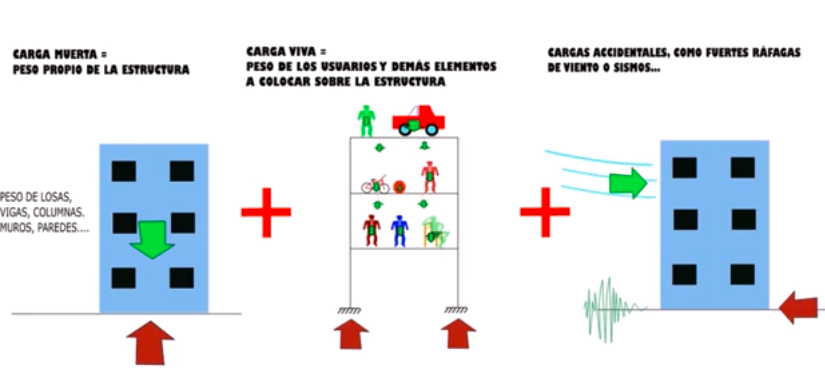
\includegraphics[width=0.7\linewidth]{im5}
	\end{center}
	
	
	
	
	\subsection{Combinaciones de Carga para Diseño (LFRD)}
	Para el método de \textbf{Diseño por Factores de Carga y Resistencia (LRFD)}, las acciones deben multiplicarse por factores de amplificación que consideran la incertidumbre estadística de su ocurrencia simultánea .. Las combinaciones fundamentales exigidas por la norma incluyen:
	
	\begin{equation}
		U = 1.4D
	\end{equation}
	\begin{equation}
		U = 1.2D + 1.6L + 0.5(L_r \text{ o } C_v)
	\end{equation}
	\begin{equation}
		U = 1.2D + 1.6(L_r \text{ o } C_v) + (L \text{ o } 0.5W)
	\end{equation}
	\begin{equation}
		U = 1.2D + 1.0W + L + 0.5(L_r \text{ o } C_v)
	\end{equation}
	\begin{equation}
		U = 1.2D + 1.0E + L + 0.2C_v
	\end{equation}
	\begin{equation}
		U = 0.9D + 1.0W
	\end{equation}
	\begin{equation}
		U = 0.9D + 1.0E
	\end{equation}
	
	\subsection{Determinación de la Masa Sísmica Efectiva ($W_s$)}
	Un aspecto crítico en la normativa de AGIES es que el sismo no se combina con la totalidad de la carga viva ordinaria, ya que estadísticamente es improbable que el edificio esté ocupado a su máxima capacidad de diseño durante el movimiento telúrico .. Por lo tanto, para el cálculo de las fuerzas sísmicas de inercia, la masa sísmica efectiva ($W_s$) debe estar constituida por:
	
	\begin{enumerate}
		\item El \textbf{100\%} de la Carga Muerta total ($D$) de la edificación ..
		\item En áreas utilizadas para almacenamiento o bodegas, se debe incluir obligatoriamente al menos un \textbf{25\%} de la Carga Viva de diseño ($L$), debido al carácter semipermanente de los bienes almacenados.
		\item En techos donde la configuración geométrica propicie la retención de ceniza volcánica, se debe incorporar la fracción correspondiente exigida por las demandas de sitio.
	\end{enumerate}

	

	%%%%%%%%%%%%%%%%%%%%%%%%%%%%%%%%%%%%%%%%%%%%%%%%%%%%%
	
	

	\section{ Irregularidades en Planta y Elevación }
	
	El diseño estructural y sismo-resistente en Guatemala se rige bajo las normativas de la \textbf{Asociación Guatemalteca de Ingeniería Estructural y Sísmica (AGIES)}. Dentro de estas regulaciones, la norma \textbf{AGIES NSE 3 (Edición 2024)} aborda de forma exhaustiva el impacto de las irregularidades en planta y en elevación en el comportamiento dinámico de las edificaciones. 
	
	Las asimetrías e irregularidades geométricas alteran el flujo correcto de las fuerzas inducidas por un sismo, concentrando el daño destructivo en puntos débiles de la edificación. Por esta razón, la normativa penaliza el uso de configuraciones complejas exigiendo análisis más rigurosos, incrementando las fuerzas de diseño o, en casos extremos de alta sismicidad, prohibiéndolas por completo.
	
	\subsection{Estructuras con Irregularidades en Planta (Capítulo 1.8)}
	Se determina que una edificación posee irregularidades en planta cuando cumple con una o más de las condiciones tipificadas por la norma en la \textbf{Tabla 1.8-1 de la NSE 3}. Estas configuraciones rompen la simetría horizontal del edificio:
	
	\begin{itemize}
		\item \textbf{Irregularidades Torsionales (H1-A y H1-B):} Ocurren cuando el centro de masa de los pisos no coincide con su centro de rigidez lateral. Al impactar el sismo, la estructura no solo se desplaza hacia los lados, sino que tiende a rotar sobre su propio eje vertical, amplificando críticamente los esfuerzos en las esquinas y columnas perimetrales.
		
		
		\begin{center}
			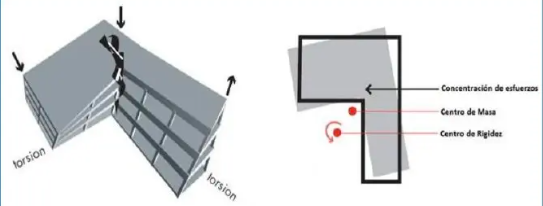
\includegraphics[width=0.7\linewidth]{im6}
		\end{center}
		
		
		
		
		\item \textbf{Esquinas Entrantes (H2):} Esta irregularidad se tipifica cuando las proyecciones de una estructura presentan entrantes en forma de ``L'', ``H'', ``U'' o ``T'' cuyos reentrantes superan el \textbf{15\%} de la dimensión total de la planta en esa dirección. Las esquinas interiores tienden a sufrir concentraciones severas de esfuerzos de desgarro lateral.
		
		\begin{center}
			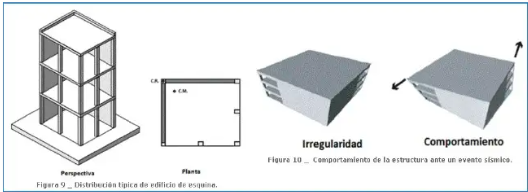
\includegraphics[width=0.7\linewidth]{im7}
		\end{center}
		
		
		
		
		
		\item \textbf{Diafragma Discontinuo (H3):} Se produce cuando los elementos horizontales (las losas de entrepiso) tienen aberturas o huecos que superan el \textbf{25\%} del área total del rectángulo que circunscribe al piso, o cuando la rigidez del diafragma varía en más de un \textbf{50\%} de un nivel a otro. Esto debilita la capacidad de las losas de transmitir uniformemente las fuerzas del sismo a los marcos o muros de carga.
		\item \textbf{Interrupción de Soportes Verticales / Desvío del Plano Lateral (H4):} Sucede cuando hay desalineaciones en el plano de los elementos verticales que resisten las fuerzas sísmicas (como un muro estructural que se corta o desplaza horizontalmente de un piso a otro), obligando a que las cargas se desvíen de su trayectoria natural.
		\item \textbf{Sistemas con Ejes No Paralelos (H5):} Se manifiesta cuando los elementos verticales sismo-resistentes principales están dispuestos de forma inclinada u oblicua respecto a la retícula estructural ortogonal (Ejes X e Y) del edificio. Al no estar alineados, el sismo genera respuestas combinadas difíciles de predecir y torsiones complejas.
	\end{itemize}
	
	\subsection{Irregularidades en Elevación (Capítulo 1.9)}
	Estas irregularidades analizan los cambios bruscos en la rigidez, masa o resistencia a lo largo de la altura del edificio, detalladas en la \textbf{Tabla 1.9-1 de la NSE 3}:
	
	\begin{itemize}
		\item \textbf{Piso Flexible / Piso Blando (V1-A y V1-B):} Un nivel se califica como ``piso flexible'' cuando su rigidez lateral es menor al \textbf{70\%} de la rigidez del piso inmediatamente superior, o menor al \textbf{80\%} del promedio de rigidez de los tres niveles encima. El caso extremo (\textbf{V1-B}) se da si la rigidez baja del \textbf{60\%} (respecto al nivel superior) o del \textbf{70\%} (respecto al promedio de los tres superiores). Es común en edificios con plantas bajas libres para comercios o estacionamientos, provocando que toda la deformación sísmica se concentre peligrosamente en ese único nivel.
		\item \textbf{Irregularidad de Masa / Peso (V2):} Ocurre cuando la masa efectiva de cualquier piso es más del \textbf{150\%} de la masa de un piso adyacente (sin contar los techos). Las variaciones severas de peso alteran bruscamente los modos de vibrar del edificio.
		\item \textbf{Geometría Vertical Inclinada / Retranqueos (V3):} Aplica si la dimensión horizontal del sistema sismo-resistente en cualquier piso supera el \textbf{130\%} de la del piso adyacente. Los cambios bruscos de sección vertical interrumpen la fluidez de las fuerzas de corte.
		\item \textbf{Discontinuidad en el Plano de Elementos Verticales (V4 y V5):} Se da cuando se interrumpen columnas, pilares o muros estructurales de manera que no continúan directamente hacia la cimentación, debiendo apoyarse sobre vigas o losas de transferencia estructural. 
		\item \textbf{Discontinuidad en la Resistencia Lateral / Piso Débil (V6 y V7):} Existe cuando la resistencia de un entrepiso ante cortante sísmico es inferior a la del nivel superior. Un ``piso extremadamente débil'' (\textbf{V7}) ocurre cuando la resistencia total es menor al \textbf{65\%} de la del nivel de arriba.
	\end{itemize}
	
	\subsection{Consecuencias y Castigos Normativos de AGIES 2024}
	Para contrarrestar el peligro que conllevan estas configuraciones, la norma AGIES impone estrictas medidas y penalizaciones de diseño:
	
	\begin{enumerate}
		\item \textbf{Uso Obligatorio de Análisis Dinámicos:} Las edificaciones que tengan irregularidades verticales o en planta no pueden diseñarse utilizando únicamente el método estático simplificado; se exige mandatoriamente un \textbf{análisis dinámico tridimensional} computarizado para capturar con precisión los efectos de torsión y vibración real.
		\item \textbf{Penalización en las Fuerzas de Diseño (Factor $\rho$):} Ciertas irregularidades de piso flexible o falta de redundancia incrementan automáticamente el factor de redundancia sísmica ($\rho$), obligando a diseñar el edificio para absorber fuerzas sísmicas mayores.
		\item \textbf{Amplificación de Torsión Accidental:} Si se detectan irregularidades torsionales severas en determinados Niveles de Protección Sísmica (NPS), los ingenieros deben obligar al modelo informático a incorporar un \textbf{10\% de excentricidad accidental} adicional como factor de seguridad.
		\item \textbf{Uso del Factor de Sobre-resistencia ($\Omega_r$):} En elementos críticos como las vigas o losas donde se interrumpen columnas estructurales (irregularidades H4 y V4), las combinaciones de carga sísmica deben ser multiplicadas por el \textbf{Factor de Incremento de Resistencia $\Omega_r$}. Esto garantiza que estos elementos de transferencia sean sumamente robustos, ya que su fallo implicaría un colapso progresivo catastrófico. Además, se exige advertir explícitamente en los planos que estas zonas son propensas a daños severos no reparables bajo sismos extremos.
		\item \textbf{Prohibiciones Absolutas:} Dependiendo del Nivel de Protección Sísmica del proyecto (NPS), ciertas irregularidades extremas —como los pisos extremadamente débiles (V7) o las irregularidades torsionales agudas (H1-B)— están \textbf{completamente prohibidas} por la normativa para evitar catástrofes estructurales.
	\end{enumerate}
	
	
	\section{Ejemplos sobre Irregularidades Estructurales }
	
	Con base en la documentación técnica analizada, se presentan a continuación ejemplos prácticos y la descripción analítica de cómo se manifiestan y evalúan cuantitativamente las irregularidades en planta y elevación en proyectos de edificación según los criterios de la \textbf{NSE 3-2024}.
	
	\subsection{Ejemplos de Irregularidades en Planta}
	
	\begin{itemize}
		\item \textbf{Ejemplo de Irregularidad Torsional Extrema (H1-B):} 
		Considere un edificio comercial asimétrico de tres niveles con forma rectangular, donde uno de los extremos laterales está compuesto enteramente por muros de corte de concreto reforzado y el extremo opuesto cuenta únicamente con marcos rígidos y ventanales diáfanos. 
		Al realizar el análisis computarizado, la aplicación de la fuerza sísmica lateral genera que el desplazamiento en el extremo flexible ($ \Delta_{max} $) sea significativamente mayor que el del extremo rígido ($ \Delta_{min} $). Si el análisis demuestra que el desplazamiento máximo supera el \textbf{40\%} del desplazamiento promedio de los dos extremos ($ \Delta_{max} > 1.4 \times \Delta_{prom} $), la estructura clasifica automáticamente como irregularidad torsional extrema .. En Guatemala, esta condición queda estrictamente prohibida para proyectos con Nivel de Protección Sísmica E (NPS E).
		
		\begin{center}
			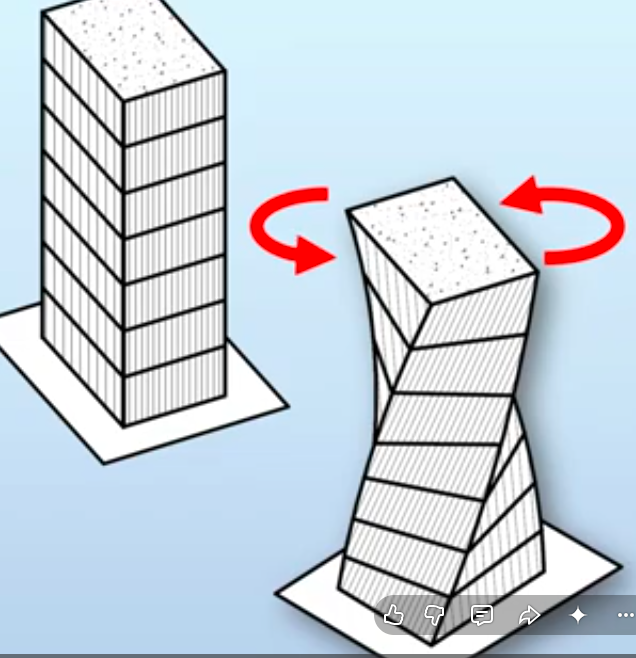
\includegraphics[width=0.5\linewidth]{im8}
		\end{center}
		
		
		\item \textbf{Ejemplo de Esquina Entrante (H2):}
		Imagínese un centro educativo diseñado con una planta arquitectónica en forma de ``L''. Si la longitud total del edificio en el eje X es de 40 metros y el bloque reentrante tiene una longitud de 8 metros en esa misma dirección, se realiza la evaluación porcentual:
		\[ \frac{8\text{ m}}{40\text{ m}} = 20\% \]
		Dado que el reentrante ($20\%$) es mayor al \textbf{15\%} de la dimensión total de la planta exigido como límite por la norma, el edificio se tipifica formalmente con irregularidad H2 .. Esto obliga al diseñador a incrementar en un 25\% las fuerzas de diseño en las conexiones entre el diafragma de la losa y los elementos verticales de soporte (columnas o muros) para los niveles de protección C, D y E ..
		
		\item \textbf{Ejemplo de Diafragma Discontinuo (H3):}
		Considere una torre de oficinas de $20 \times 30$ metros (área total circunscrita de $600\text{ m}^2$) que incorpora un gran pozo de luz central o ducto de ascensores y gradas con unas dimensiones de $10 \times 16$ metros. El área total del vacío en la losa corresponde a $160\text{ m}^2$. Al evaluar el cumplimiento:
		\[ \frac{160\text{ m}^2}{600\text{ m}^2} = 26.67\% \]
		Debido a que el área de la abertura supera el \textbf{25\%} del área total del diafragma, la estructura califica con irregularidad H3 .. El diafragma pierde la capacidad de comportarse de manera completamente rígida, exigiendo análisis dinámicos tridimensionales específicos para simular la flexibilidad real de la losa ..
	\end{itemize}
	
	\subsection{Ejemplos de Irregularidades en Elevación}
	
	\begin{itemize}
		\item \textbf{Ejemplo de Piso Flexible / Piso Blando (V1-A y V1-B):}
		Un caso muy común en el contexto urbano de Guatemala son los edificios de apartamentos de múltiples niveles que utilizan el primer nivel exclusivamente como estacionamiento o recepción (planta libre con columnas delgadas y sin muros), mientras que los niveles superiores poseen una gran densidad de muros divisorios de mampostería o concreto. 
		Si la rigidez lateral calculada del primer nivel es de $35,000\text{ kN/m}$ y la rigidez del segundo nivel es de $60,000\text{ kN/m}$, evaluamos la relación de rigidez:
		\[ \frac{35,000}{60,000} = 58.33\% \]
		Al ser menor al \textbf{60\%} de la rigidez del piso inmediatamente superior, el edificio clasifica como un caso extremo de Piso Flexible (\textbf{V1-B}) .. La normativa penaliza este diseño obligando a aplicar un factor de redundancia incremental de $\rho = 1.10$ sobre las fuerzas de diseño ..
		
		\item \textbf{Ejemplo de Interrupción de Soportes Verticales (V4):}
		Un ejemplo clásico ocurre en hoteles o centros de convenciones donde las columnas del núcleo central del edificio descienden normalmente desde el cuarto piso hasta el segundo nivel, pero en el primer nivel se requiere un gran salón de eventos sin columnas intermedias. Para lograrlo, las columnas superiores se interrumpen y se hacen descansar sobre una robusta viga de gran peralte o ``viga de transferencia'' en el techo del primer nivel ..
		La norma AGIES clasifica esto como una discontinuidad severa en la ruta de las cargas (V4) .. Como castigo y medida de seguridad extrema ante el colapso, exige que las vigas de transferencia y las columnas que reciben esa carga concentrada se diseñen amplificando los efectos sísmicos por el \textbf{Factor de Sobre-resistencia $\Omega_r$} (típicamente $\Omega_r = 3$) ..
		
		\item \textbf{Ejemplo de Piso Débil (V6 y V7):}
		Se evalúa un edificio donde la resistencia total al cortante de las columnas del tercer nivel es de $800\text{ kN}$, mientras que la resistencia al cortante del cuarto nivel es de $1,300\text{ kN}$. Al calcular la proporción de resistencia:
		\[ \frac{800\text{ kN}}{1,300\text{ kN}} = 61.54\% \]
		Como la resistencia del tercer nivel es menor al \textbf{65\%} de la del nivel superior, se clasifica como una discontinuidad en la resistencia lateral bajo la categoría de \textbf{Piso Extremadamente Débil (V7)} .. Bajo la normativa AGIES 2024, esta condición está rotundamente prohibida para edificaciones que se ubiquen en zonas de alta sismicidad catalogadas con NPS C, D y E ..
	\end{itemize}
	
	
	
	
	\section{Redundancia Estructural}
	
	La redundancia estructural es definida en la normativa guatemalteca como el mecanismo principal de supervivencia de una edificación ante la demanda de cargas laterales extremas, tales como las inducidas por un evento sísmico. Este concepto representa la capacidad intrínseca que posee un sistema estructural para redistribuir los esfuerzos de manera segura hacia otras líneas de defensa cuando uno o varios de sus componentes principales (como una columna o un muro de carga) experimentan una falla o alcanzan su límite elástico .. 
	
	El objetivo fundamental de exigir condiciones de redundancia es evitar a toda costa el \textbf{colapso progresivo}, garantizando que la estructura cuente con múltiples rutas alternas de transmisión de carga para absorber y disipar la energía sísmica de forma hiperestática ..
	
	\subsection{El Factor de Redundancia ($\rho$)}
	La norma \textbf{AGIES NSE 3-2024} cuantifica y penaliza la falta de líneas de defensa en el diseño sísmico a través del coeficiente denominado \textbf{Factor de Redundancia ($\rho$)}. Este factor actúa directamente como un multiplicador de las fuerzas sísmicas horizontales de diseño en el espectro de respuesta. El valor del coeficiente $\rho$ se asigna según las siguientes condiciones reglamentarias:
	
	\begin{itemize}
		\item \textbf{$\rho = 1.00$ (Sistemas Redundantes):} Se aplica a edificaciones que poseen un número suficiente de marcos, columnas o muros estructurales dispuestos de tal forma que la falla de un elemento individual no comprometa la estabilidad global de la estructura. Bajo este escenario, no se genera ningún incremento en las fuerzas sísmicas actuantes.
		\item \textbf{$\rho = 1.10$ (Sistemas No Redundantes / Penalizados):} Se asigna obligatoriamente a aquellas estructuras que dependen de muy pocas líneas de defensa para resistir las solicitaciones sísmicas. Al utilizar este factor, la norma incrementa las fuerzas sísmicas de diseño en un \textbf{10\%}, forzando a que los elementos existentes sean calculados con secciones y armaduras más robustas para mitigar el riesgo intrínseco de su configuración ..
	\end{itemize}
	
	\subsection{Criterios de Evaluación y Límites Normativos}
	Para determinar la obligatoriedad de la penalización por redundancia, el ingeniero calculista debe evaluar analíticamente cada nivel o entrepiso de la edificación en ambas direcciones ortogonales de análisis (Eje X y Eje Y), sometiendo el sistema sismo-resistente a los siguientes criterios de remoción virtual:
	
	\begin{enumerate}
		\item \textbf{Evaluación en Marcos Rígidos:} Se debe verificar el impacto de remover la contribución a flexión y corte de una columna o de las conexiones de una viga en el perímetro. Si la supresión de dicho elemento reduce la resistencia lateral total del entrepiso en más de un \textbf{33\%}, o si induce una irregularidad de tipo torsional extrema (H1-B), el sistema completo en esa dirección se tipifica como no redundante.
		\item \textbf{Evaluación en Muros de Corte o Marcos Arriostrados:} Se analiza el efecto de la pérdida de un tramo de muro estructural o de un elemento de arriostramiento diagonal. Si la eliminación de dicha línea de defensa provoca una reducción superior al \textbf{33\%} en la capacidad de corte basal del entrepiso, o genera una excentricidad que active la irregularidad H1-B, el entrepiso completo se penaliza con el factor $\rho = 1.10$.
	\end{enumerate}
	
	\subsection{Filosofía de Múltiples Líneas de Defensa}
	La normativa técnica de AGIES enfatiza que la simplicidad y la correcta estructuración hiperestática son los pilares fundamentales para la seguridad de los ocupantes y la resiliencia económica de la obra .. Diseñar bajo el concepto de redundancia implica configurar \textbf{múltiples líneas de defensa} paralelas y conectadas de forma solidaria .. La ingeniería sismo-resistente moderna prefiere evitar la concentración de cargas en un número reducido de elementos masivos, favoreciendo en su lugar la distribución de las solicitaciones en una red densa de pórticos o muros acoplados que aseguren una disipación de energía uniforme y eviten fallas frágiles súbitas.
	
	
	
	
	%%%%%%%%%%%%%%%%%%%%%%%%%%%%%%%%%%%%%%%%%%%%%%%%555
	
		\newpage
	
	% ----------------------------------

	\section{Conclusión}
	
	Por lo tanto el diseño sismo-resistente en Guatemala, fundamentado en las normas AGIES, integra criterios de seguridad, funcionalidad y resiliencia estructural. La adecuada clasificación de las obras, junto con la correcta evaluación y combinación de cargas, permite establecer niveles de diseño acordes a la importancia y uso de cada edificación. 
	
	Asimismo, el control de irregularidades en planta y elevación resulta fundamental para evitar concentraciones de esfuerzos y mejorar el comportamiento dinámico ante sismos. Finalmente, la redundancia estructural se consolida como un elemento clave para prevenir fallas críticas, asegurando edificaciones más estables y seguras que protejan la vida humana frente a eventos sísmicos.
	




	
	% ----------------------------------
	%         BIBLIOGRAFÍA APA
	% ----------------------------------
	\newpage

	
	\bibliographystyle{apacite}
\renewcommand{\refname}{Referencias}

\bibliography{bibliografia}


\renewcommand{\refname}{Referencias}




	Asociación Guatemalteca de Ingeniería Estructural y Sísmica. (2024). \textit{Normas de Seguridad Estructural para Guatemala. NSE 1: Generalidades, administración de las normas y supervisión técnica} (Edición 2024). AGIES.
	
	Asociación Guatemalteca de Ingeniería Estructural y Sísmica. (2024). \textit{Normas de Seguridad Estructural para Guatemala. NSE 2: Demandas estructurales y condiciones de sitio} (Edición 2024). AGIES.
	
	Asociación Guatemalteca de Ingeniería Estructural y Sísmica. (2024). \textit{Normas de Seguridad Estructural para Guatemala. NSE 2.1: Estudios geotécnicos} (Edición 2024, Versión Beta). AGIES.
	
	Asociación Guatemalteca de Ingeniería Estructural y Sísmica. (2024). \textit{Normas de Seguridad Estructural para Guatemala. NSE 3: Diseño estructural de edificaciones} (Edición 2024). AGIES.
	


		
	
	
	
\end{document}